This chapter introduces the datasets and metrics we used.

\section{Winoground}

\subsection{Dataset}

See \cref{tab:stats-tag-subset}

See \cref{fig:dataset-examples-linguistic} and \cref{fig:dataset-examples-visual}

\begin{table}
\centering
\begin{tabular}{lrr}
\toprule
 Category & Tag    &   Count \\
\midrule
 %All Examples & 400\\
 & Object   &     141 \\
 Linguistic$_\text{swap-dep.}$ & Relation &     233 \\
 & Both &      26 \\\midrule
 Linguistic$_\text{swap-indep.}$ & 1 Main Pred & 293 \\
 & 2 Main Preds & 108 \\\midrule
 & Symbolic &  41 \\
 Visual & Series &  31 \\
 & Pragmatics &  24\\
\bottomrule
\end{tabular}
\caption{Linguistic and visual tag counts in the Winoground dataset. Every example has a linguistic tag; only examples that contain the visual phenomena have visual tags.}
\label{tab:stats-tag-subset}
\end{table}

\begin{figure}
\centering
    \begin{minipage}[t]{.30\textwidth}
        \begin{subfigure}[t]{\textwidth}
        \centering
        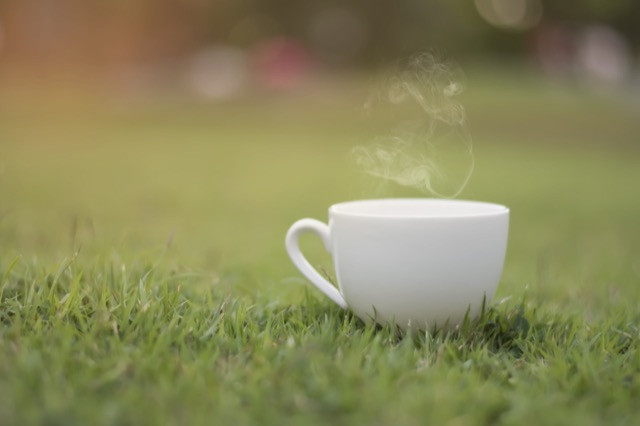
\includegraphics[height=3cm]{ex_14_img_0.png}
        \caption{there is [a mug] in [some grass]}
        \end{subfigure}\\
        \begin{subfigure}[t]{\textwidth}
        \centering
        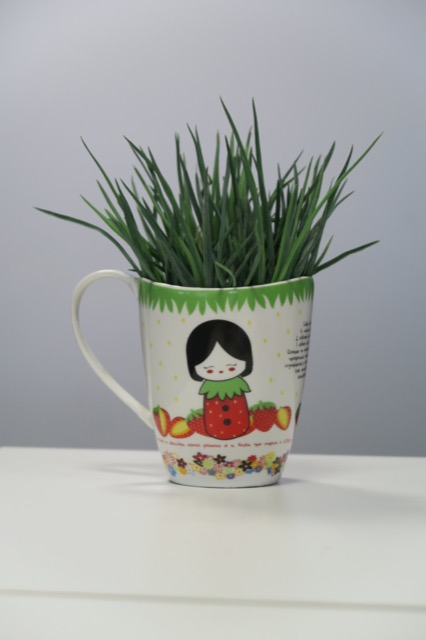
\includegraphics[height=3cm]{ex_14_img_1.png}
        \caption{there is [some grass] in [a mug]}
        \end{subfigure}%    
        \caption*{\textit{Object}}
    \end{minipage}
    \hfill
    \begin{minipage}[t]{.30\textwidth}
        \begin{subfigure}[t]{\textwidth}
        \centering
        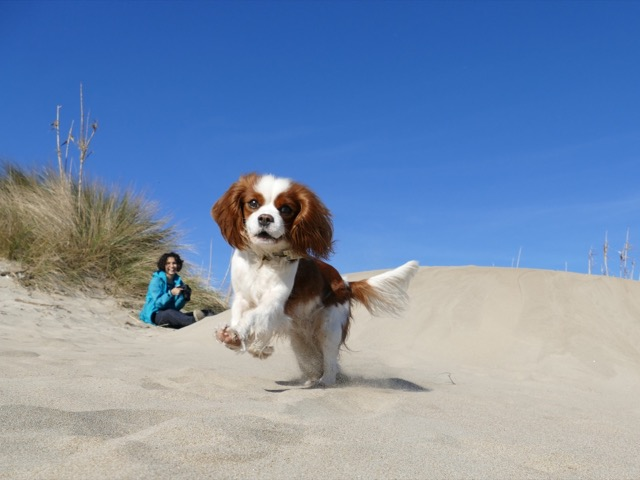
\includegraphics[height=3cm]{ex_21_img_0.png}
        \caption{a person [sits] and a dog [stands]}
        \end{subfigure}\\
        \begin{subfigure}[t]{\textwidth}
        \centering
        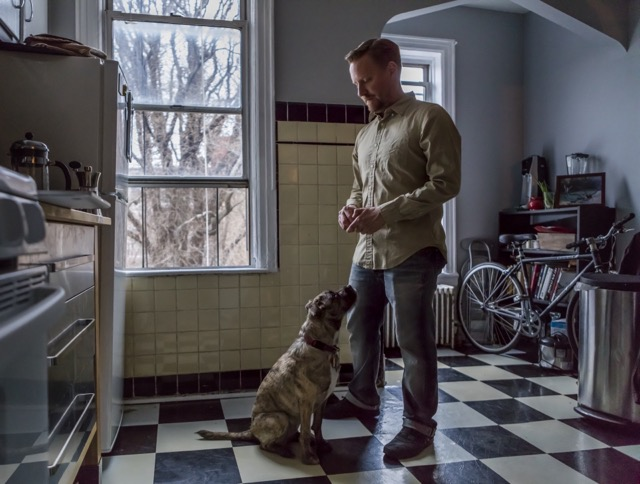
\includegraphics[height=3cm]{ex_21_img_1.png}
        \caption{a person [stands] and a dog [sits]}
        \end{subfigure}%    
        \caption*{\textit{Relation}}
    \end{minipage}
    \hfill
    \begin{minipage}[t]{.30\textwidth}
        \begin{subfigure}[t]{\textwidth}
        \centering
        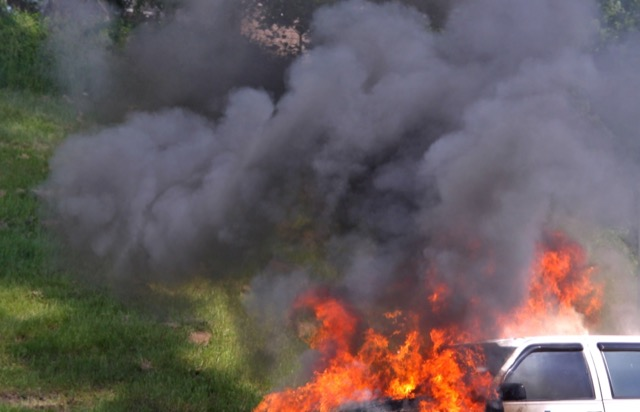
\includegraphics[height=3cm]{ex_72_img_1.png}
        \caption{it's a [truck] [fire]}
        \end{subfigure}\\
        \begin{subfigure}[t]{\textwidth}
        \centering
        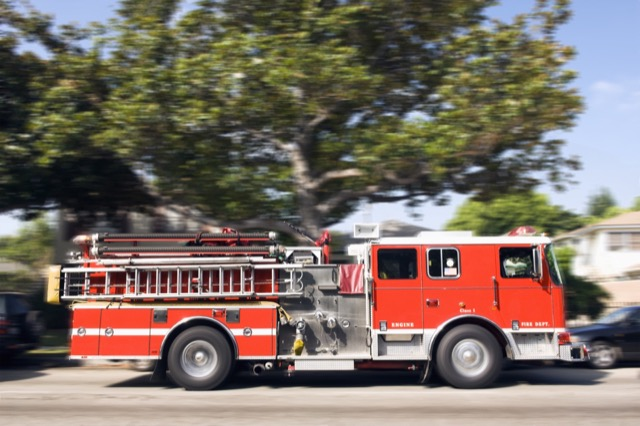
\includegraphics[height=3cm]{ex_72_img_0.png}
        \caption{it's a [fire] [truck]}
        \end{subfigure}%
        \caption*{\textit{Both}}
    \end{minipage}%
    \caption[]{Examples from the dataset for the swap-dependent linguistic tags \textit{Object}, \textit{Relation} and \textit{Both} from left to right. The linguistic examples are additionally tagged with 2, 1, and 1 main predicates from left to right.}
    \label{fig:dataset-examples-linguistic}
\end{figure}

\begin{figure}
\centering
    \begin{minipage}{.30\textwidth}
        \begin{subfigure}{\textwidth}
        \centering
        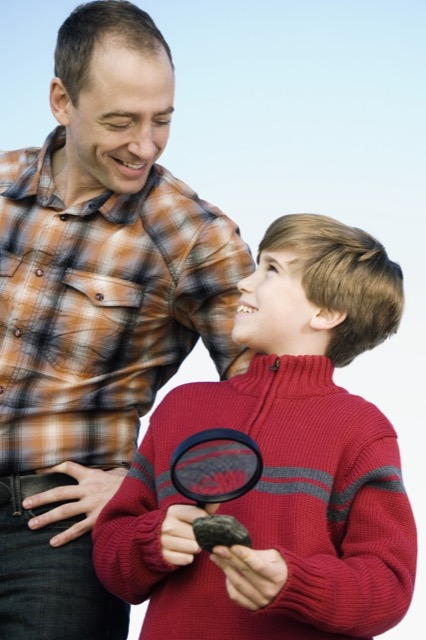
\includegraphics[height=3cm]{ex_75_img_0.png}
        \caption{the kid [with the magnifying glass] looks at them []}
        \end{subfigure}\\
        \begin{subfigure}{\textwidth}
        \centering
        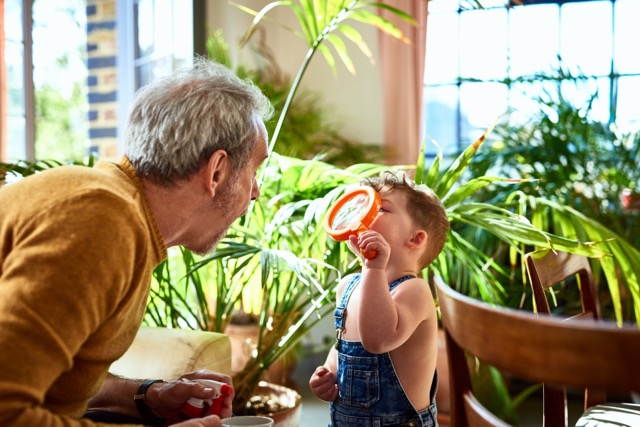
\includegraphics[height=3cm]{ex_75_img_1.png}
        \caption{the kid [] looks at them [with the magnifying glass]}
        \end{subfigure}%    
        \caption*{\textit{Pragmatics}}
    \end{minipage}
    \hfill
    \begin{minipage}{.30\textwidth}
        \begin{subfigure}{\textwidth}
        \centering
        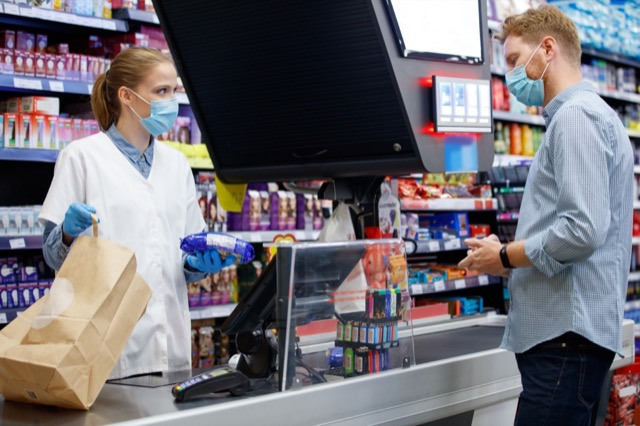
\includegraphics[height=3cm]{ex_27_img_0.png}
        \caption{the person with the ponytail [packs] stuff and other [buys] it}
        \end{subfigure}\\
        \begin{subfigure}{\textwidth}
        \centering
        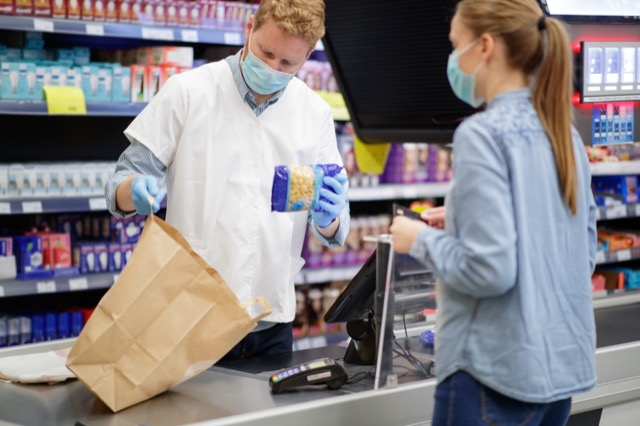
\includegraphics[height=3cm]{ex_27_img_1.png}
        \caption{the person with the ponytail [buys] stuff and other [packs] it}
        \end{subfigure}%    
        \caption*{\textit{Series}}
    \end{minipage}
    \hfill
    \begin{minipage}{.30\textwidth}
        \begin{subfigure}{\textwidth}
        \centering
        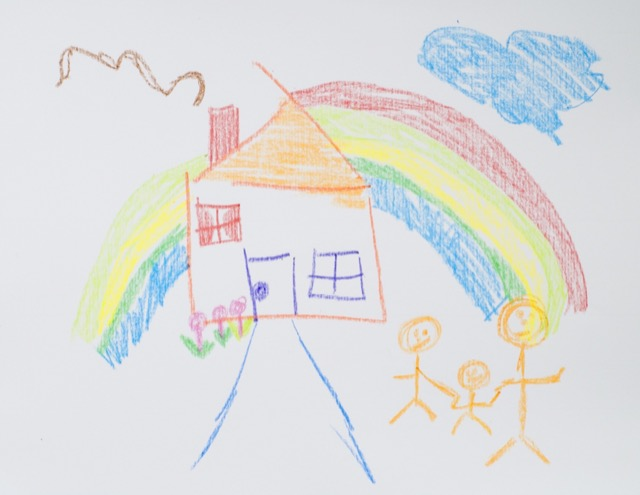
\includegraphics[height=3cm]{ex_61_img_0.png}
        \caption{there are [three] people and [two] windows}
        \end{subfigure}\\
        \begin{subfigure}{\textwidth}
        \centering
        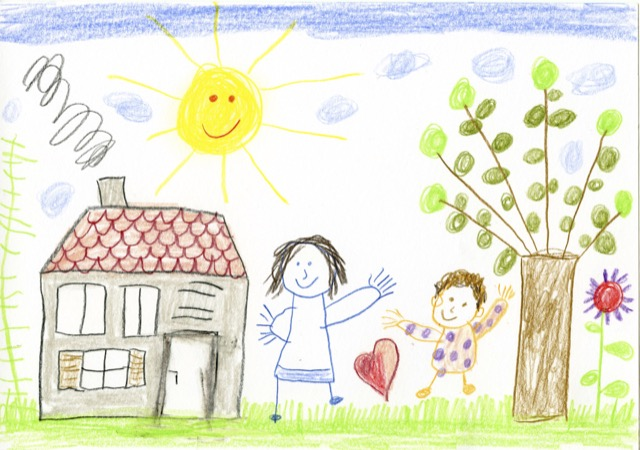
\includegraphics[height=3cm]{ex_61_img_1.png}
        \caption{there are [two] people and [three] windows}
        \end{subfigure}%    
        \caption*{\textit{Symbolic}}
    \end{minipage}
    \caption[]{Examples from the dataset for the swap-dependent visual tags \textit{Pragmatics}, \textit{Series} and \textit{Symbolic} from left to right. The visual examples are additionally tagged with the \textit{Relation} tag, and 1, 2, and 1 main predicates from left to right.}
    \label{fig:dataset-examples-visual}
\end{figure}

\subsection{Metrics}

\subsubsection{Score}

Performance on Winoground \cite{thrush2022winoground} is computed according to three different metrics that evaluate different aspects of the models' visio-linguistic reasoning abilities.

The first metric is the \textbf{text score}, which measures whether a model can select the correct caption, given an image. 
Given images $I_0$ and $I_{1}$ and captions $C_{0}$ and $C_{1}$, the text score for an example $(C_{0},I_{0},C_{1},I_{1})$ is computed according to:
\begin{equation}\label{eq:text-score}
        ts(C_{0},I_{0},C_{1},I_{1})= 
    \begin{cases}
        1 & \text{if}\  s(C_{0}, I_{0}) > s(C_{1}, I_{0}) \\
        & \ \ \text{and}\ s(C_{1}, I_{1}) > s(C_{0}, I_{1}) \\
        0              & \text{otherwise}
    \end{cases}
\end{equation}
where $s(\cdot)$ is the model's score for the image/caption pair.

The second metric is the \textbf{image score}, which measures whether a model can select the correct image, given a caption.
The image score for an example is computed according to:
\begin{equation}\label{eq:image-score}
        is(C_{0},I_{0},C_{1},I_{1})= 
    \begin{cases}
        1 & \text{if}\  s(C_{0}, I_{0}) > s(C_{0}, I_{1})\\
        & \ \ \text{and}\ s(C_{1}, I_{1}) > s(C_{1}, I_{0}) \\
        0              & \text{otherwise}
    \end{cases}
\end{equation}

Our final metric \textbf{group score} combines the previous two, which measures if every combination for a given example is correctly scored by the model.
The group score for an example is computed according to:
\begin{equation}\label{eq:group-score}
        gs(C_{0},I_{0},C_{1},I_{1})= 
    \begin{cases}
        1 & \text{if}\  ts(C_{0},I_{0},C_{1},I_{1})  \\
         & \ \ \text{and}\ is(C_{0},I_{0},C_{1},I_{1})\\
        0              & \text{otherwise}
    \end{cases}
\end{equation}

\subsubsection{Accuracy}

We also add three additional accuracy metrics. These are similar to the previous ones, but accuracy is 0.5 when one of the pairs is correct.

Given images $I_0$ and $I_{1}$ and captions $C_{0}$ and $C_{1}$, the \textbf{text accuracy} for an example $(C_{0},I_{0},C_{1},I_{1})$ is computed according to:
\begin{equation}\label{eq:text-accuracy}
        ta(C_{0},I_{0},C_{1},I_{1})= 
    \begin{cases}
        1 & \text{if}\  s(C_{0}, I_{0}) > s(C_{1}, I_{0}) \\
        & \ \ \text{and}\ s(C_{1}, I_{1}) > s(C_{0}, I_{1}) \\
        0.5 & \text{if}\  s(C_{0}, I_{0}) > s(C_{1}, I_{0}) \\
        & \ \ \text{xor}\ s(C_{1}, I_{1}) > s(C_{0}, I_{1}) \\
        0              & \text{otherwise}
    \end{cases}
\end{equation}
where $s(\cdot)$ is the model's score for the image/caption pair.

The \textbf{image accuracy} for an example is computed according to:
\begin{equation}\label{eq:image-accuracy}
        ia(C_{0},I_{0},C_{1},I_{1})= 
    \begin{cases}
        1 & \text{if}\  s(C_{0}, I_{0}) > s(C_{0}, I_{1})\\
        & \ \ \text{and}\ s(C_{1}, I_{1}) > s(C_{1}, I_{0}) \\
        0.5 & \text{if}\  s(C_{0}, I_{0}) > s(C_{0}, I_{1})\\
        & \ \ \text{xor}\ s(C_{1}, I_{1}) > s(C_{1}, I_{0}) \\
        0              & \text{otherwise}
    \end{cases}
\end{equation}

The \textbf{group accuracy} in our framework is computed according to:
\begin{equation}\label{eq:group-accuracy}
        ga(C_{0},I_{0},C_{1},I_{1})= 
        (ta(C_{0},I_{0},C_{1},I_{1}) + ia(C_{0},I_{0},C_{1},I_{1})) / 2\\
\end{equation}

\section{Visual Spatial Reasoning}